% ICBET 2026 — Beamer Presentation
% "Towards a Human-Guided AutoML Application for Democratizing
%  Predictive Modeling in Clinical Research"
% Compile: pdflatex main.tex  (run twice)
% ─────────────────────────────────────────────────────────────────────────────
\documentclass[aspectratio=169,10pt,english,dvipsnames]{beamer}

% Pacotes
\usepackage{lipsum}
\usepackage{graphicx}
\usepackage{color}
\usepackage[table]{xcolor}
\usepackage{tikz}
\usepackage{tcolorbox}
\usepackage{amsmath}
\usepackage{amsfonts}
\usepackage{amssymb}
\usepackage{mathrsfs}
\usepackage{mathtools}
\usepackage{enumitem} 
\usepackage{float}
\usepackage[utf8]{inputenc}	

\usepackage{caption}

\usepackage[spanish, es-tabla]{babel}
\usepackage[babel, spanish=spanish]{csquotes}
\AtBeginEnvironment{quote}{\small}
\decimalpoint

\usetikzlibrary{decorations.pathreplacing,calc}
\usetikzlibrary{shadows}
\usetikzlibrary{positioning}

\usepackage{booktabs}

\usepackage{subcaption}

\usepackage{multicol}

\usepackage{multirow}


% Theme choice:
\usetheme{CambridgeUS}

% Cores personalizadas
\definecolor{PROFMATgreen}{RGB}{0, 138, 163}
\definecolor{UFTgreen}{RGB}{0, 137, 124}
\definecolor{UFTblue}{RGB}{0, 84, 132}
\definecolor{UFTyellow}{RGB}{253, 185, 46}
\definecolor{UFTgray}{RGB}{132, 134, 136}

\definecolor{UC}{RGB}{0,178,169}

% Ativar numeração de tabelas
\setbeamertemplate{caption}[numbered]

% Definir novo estilo de item com quadrado verde
\setlist[itemize,1]{label=\textcolor{UFTgreen}{\rule{1ex}{1ex}}}

\setbeamercolor*{structure}{bg=UFTgreen,fg=black}

\setbeamercolor*{palette primary}{fg=black,bg=PROFMATgreen}
\setbeamercolor*{palette secondary}{fg=white,bg=UFTblue}
\setbeamercolor*{palette tertiary}{fg=black,bg=UFTgreen}
\setbeamercolor*{palette quaternary}{fg=white,bg=black}

\setbeamercolor{section in toc}{fg=black,bg=white}
\setbeamercolor{alerted text}{fg=white}

\setbeamercolor*{item}{fg=PROFMATgreen}

\setbeamercolor{block title}{bg=UFTgreen,fg=white}
\setbeamercolor{block body}{bg=UFTgray!10,fg=black}

\setbeamercolor{titlelike}{fg=white, bg=UFTblue}
\setbeamercolor{frametitle}{bg=UFTgray!20,fg=UFTgreen}



\setbeamertemplate{background}{
    \parbox[c][\paperheight][c]{\paperwidth}{
        \vfill
        
\includegraphics[width=\paperwidth,height=\paperheight,keepaspectratio]{img/modelo/bakcground.png} 
        \vfill
    }
}


% Personalizar portada
\setbeamertemplate{title page}{
  \begin{columns}[c,totalwidth=\paperwidth]
    \column{.05\paperwidth}
      \centering
      \raisebox{0.1cm}{%
        \parbox{.5\paperwidth}{\centering\scriptsize
        16th International Conference on Biomedical Engineering and Technology\\
        Bali, Indonesia · 12 -- 15 June, 2026}
      }
    \column{.45\paperwidth}
      \centering
      
\includegraphics[height=1.2cm]{img/UC_LogotipoPrincipal.png}
\end{columns}

  \vskip1em
  \begingroup
    \centering
    \begin{beamercolorbox}[sep=8pt,center,shadow=true,rounded=false]{title}
      \usebeamerfont{title}\inserttitle\par%
      \ifx\insertsubtitle\@empty\else
        \vskip0.25em{\usebeamerfont{subtitle}\usebeamercolor[fg]{subtitle}\insertsubtitle\par}%
      \fi
    \end{beamercolorbox}
    \vskip1em
    \begin{beamercolorbox}[sep=6pt,center]{author}\usebeamerfont{author}\insertauthor\end{beamercolorbox}
    \vskip0.2em
    \begin{beamercolorbox}[sep=5pt,center]{advisor}\usebeamerfont{institute}\advisorname\end{beamercolorbox}
    \vskip0.2em
    \begin{beamercolorbox}[sep=5pt,center]{institute}\usebeamerfont{institute}\insertinstitute\end{beamercolorbox}
    \vskip0.2em
    \begin{beamercolorbox}[sep=5pt,center]{date}\usebeamerfont{institute}\insertdate\end{beamercolorbox}
    \vskip0.5em
  \endgroup
  \vfill
}



% Remover bordas arredondadas dos blocks
\makeatletter
\setbeamertemplate{blocks}[default] % Isso remove o arredondamento
\makeatother


% Pacotes de citações
% ---

\usepackage[alf,abnt-etal-text=it,abnt-repeated-author-omit=yes,abnt-etal-list=0,abnt-etal-cite=3,abnt-emphasize=bf]{abntex2cite}	% Citações padrão ABNT



\setbeamercolor{bibliography entry author}{fg=black}
\setbeamertemplate{bibliography item}{\newblock}


\setbeamertemplate{frametitle continuation}{}

% Redefinir o separador para um traço
% Redefinir o separador
\captionsetup[figure]{labelformat=simple, labelsep=endash, textformat=period, font=footnotesize}
\captionsetup[table]{labelformat=simple, labelsep=endash, textformat=period, font=footnotesize}


% Redefine espaçamento antes e depois da legenda em figuras e tabelas
\captionsetup[figure]{aboveskip=2pt, belowskip=0pt}
\captionsetup[table]{aboveskip=2pt, belowskip=0pt}


% Define uma penalidade alta para a hifenização
\hyphenpenalty=10000
\tolerance=10000


% Personalizando o estilo da tabela de conteúdos
\setbeamertemplate{section in toc}[sections numbered]
\renewcommand{\thesection}{\textcolor{PROFMATgreen}{\arabic{section}}}
\renewcommand{\thesubsection}{\textcolor{PROFMATgreen}{\arabic{section}.\arabic{subsection}}}

\setbeamersize{text margin left=0.8cm, text margin right=0.8cm}


% ── Colour aliases (mapped to the customizacoes palette) ──────────────────────
\colorlet{UCblue}     {UFTblue}
\colorlet{UCblueLight}{PROFMATgreen}
\colorlet{UCbluePale} {UFTblue!15}
\colorlet{UCgreen}    {UFTgreen}
\colorlet{UCgray}     {UFTgray}
\definecolor{UCred}   {RGB}{180,30,30}
\definecolor{UCorange}{RGB}{210,100,0}
% ── Extra TikZ libraries not loaded in customizacoes ─────────────────────────
\usetikzlibrary{shapes.geometric,arrows.meta}
% ── Extra packages ────────────────────────────────────────────────────────────
\usepackage{array}
\usepackage{url}

\usepackage{booktabs}
\usepackage{multicol}

% ── Presentation metadata ─────────────────────────────────────────────────────
\title[HAMELIN for Clinical Research]{%
  Towards a Human-Guided AutoML Application\\
  for Democratizing Predictive Modeling in Clinical Research}

\author[Diego García-Prieto]{%
  Diego García-Prieto\inst{1} \and
  Camilo Palazuelos\inst{1} \and
  Rafael Duque\inst{1} \and
  Lucía Lavín-Alconero\inst{2}}

\institute{%
  \inst{1}Dept. of Mathematics, Statistics and Computer Science
          \textemdash{} University de Cantabria
  \and
  \inst{2}Clinical Trials Agency Valdecilla-IDIVAL
          \textemdash{} Marqués de Valdecilla University Hospital}

\date{14th June, 2026}

% ── Convenience commands ──────────────────────────────────────────────────────
\newcommand{\advisorname}{}   % required by the title page template
\newcommand{\yes}{\textcolor{UCgreen!70!black}{\checkmark}}
\newcommand{\no}{$\times$}
\newcommand{\partcheck}{$\sim$}

% ─────────────────────────────────────────────────────────────────────────────
\begin{document}

% ── Title slide ───────────────────────────────────────────────────────────────
\begin{frame}
  \titlepage
  \vspace{-4mm}
  \begin{center}
    \scriptsize
    \textit{Supported by grant PID2023-146243OB-I00 funded by MICIU/AEI and ERDF/EU}
  \end{center}
\end{frame}

% ── Table of contents ─────────────────────────────────────────────────────────
\begin{frame}[t]{Contents}
  \tableofcontents
\end{frame}

% ══════════════════════════════════════════════════════════════════════════════
\section{Motivation}
% ══════════════════════════════════════════════════════════════════════════════

\begin{frame}{Research Context} \small
  \begin{columns}[T]
    \begin{column}{0.54\textwidth}
      \begin{itemize}
        \item \textbf{AutoML democratization}:\\
          Strong need for tools reducing technical barriers in predictive modeling

        \item \textbf{Clinical ML opportunity}:\\
          Predictive models to support diagnosis, prognosis and treatment decisions

        \item \textbf{Clinical study types}:\\
          Patient registries · Observational studies · Clinical trials:\\ each with distinct protocol constraints and variable structures

        \item \textbf{Gap in practice}:\\
          Domain-agnostic tools fail in clinical settings — potential remains unrealized
      \end{itemize}
    \end{column}
    \begin{column}{0.44\textwidth}
      \begin{itemize}
        \item \textbf{HAMELIN proposal}:\\
          Protocol-aware AutoML designed for Clinical Research Professionals (CRPs)
      \end{itemize}
      \vfill
      \vspace{4mm}
      \begin{block}{Four Research Contributions}
        \begin{enumerate} \scriptsize
          \item Protocol-aware interface grounded in real clinical protocols
          \item Mapping clinical concepts to ML pipeline stages
          \item Operationalization and evaluation of HGML criteria
          \item Participatory design methodology involving CRPs
        \end{enumerate}
      \end{block}
    \end{column}
  \end{columns}
\end{frame}

\begin{frame}{The Expertise Gap} \small
  \begin{center}
    \begin{tikzpicture}[scale=0.82, transform shape]
      % Clinicians
      \node[rectangle, draw=UCblue, fill=UCbluePale, minimum width=3.2cm,
            minimum height=2.6cm, text width=3cm, align=center,
            rounded corners=0.3cm, drop shadow, font=\small] (clin) at (0,0) {
        \textbf{Clinical}\\[1mm]\textbf{Researchers}\\[3mm]
         Domain expertise\\Clinical protocols\\No ML training};
      % Data scientists
      \node[rectangle, draw=UCgreen, fill=UCgreen!15, minimum width=3.2cm,
            minimum height=2.6cm, text width=3cm, align=center,
            rounded corners=0.3cm, drop shadow, font=\small] (ds) at (9.5,0) {
        \textbf{Data}\\[1mm]\textbf{Scientists}\\[3mm]
        ML expertise\\Algorithm design\\No clinical training};
      % GAP
      \node[rectangle, draw=UCorange, dashed, fill=UCorange!8, minimum width=2.8cm,
            minimum height=2.6cm, text width=2.5cm, align=center,
            rounded corners=0.2cm, font=\small] (gap) at (4.75,0) {
        \textbf{GAP}\\[2mm]
        Terminology\\Protocol structure\\ML requirements\\Clinical validity};
      % Arrows
      \draw[->, thick, UCblue!70] (clin.east) -- (gap.west);
      \draw[->, thick, UCgreen!70] (ds.west) -- (gap.east);
      % HAMELIN bridge
      \node[rectangle, draw=UCblue, fill=UCblue, text=white,
            minimum width=5.2cm, minimum height=0.85cm,
            rounded corners=0.2cm, font=\small\bfseries] (ham) at (4.75,-2.6) {HAMELIN};
      \draw[->, thick, UCblue!80, dashed] (ham.north) -- (gap.south);
      \draw[thick, UCblue!50, dashed] (ham.west) -- +(-2.5,0) |- (clin.south);
      \draw[thick, UCgreen!50, dashed] (ham.east) -- +(2.5,0) |- (ds.south);
    \end{tikzpicture}
  \end{center}
\end{frame}

\begin{frame}{What Generic AutoML Ignores}
  Existing platforms \textbf{treat clinical datasets as generic matrices}, ignoring:
  \vspace{2mm}
  \begin{table}
    \centering \small
    \renewcommand{\arraystretch}{1.3}
    \begin{tabular}{p{3.0cm} p{4.8cm} p{4.8cm}}
      \toprule
      \textbf{Ignored Aspect} & \textbf{Clinical Significance} & \textbf{Consequence if Ignored} \\
      \midrule
      Protocol phases
        & Screening $\neq$ Follow-up data
        & \textcolor{UCred}{\textbf{Data leakage}}: variables collected \emph{after} the outcome used to predict it \\
      Endpoint hierarchy       & Primary vs.\ secondary endpoints             & Invalid conclusions \\
      Inclusion/exclusion      & Defines study population                      & Wrong population trained \\
      Confounding variables    & Influence both exposure and outcome           & \textcolor{UCred}{\textbf{Biased predictions}} \\
      Study design type        & Registry $\neq$ Trial requirements            & Methodological mismatch \\
      \bottomrule
    \end{tabular}
  \end{table}
  \vspace{2mm}
  \begin{alertblock}{Key Finding}
    No existing tool adapts to the distinct requirements of patient registries,
    observational studies and clinical trials within a unified interface.
  \end{alertblock}
\end{frame}

% ══════════════════════════════════════════════════════════════════════════════
\section{Background}
% ══════════════════════════════════════════════════════════════════════════════

\begin{frame}{Human-Centered Artificial Intelligence (HCAI)} \small
  \begin{minipage}{0.5\textwidth}
  \begin{block}{HCAI Framework (Shneiderman, 2022)}
      \begin{itemize}
        \item \textbf{Paradigm shift}:\\
        Decoupling automation from human control

        \item \textbf{Two-dimensional conception}:\\
        High automation + High human control are simultaneously achievable

        \item \textbf{Goal}:\\
        Upper-right quadrant: extensive automation with meaningful user control

      \end{itemize}
  \end{block}
      \textbf{Applied to HAMELIN}:\\
        Explicit design target. Full HCAI compliance
    \vspace{3mm}
    
    No existing tool achieves maximum on both dimensions simultaneously
  \end{minipage}%
  \begin{minipage}{0.5\textwidth}
    \centering
    \begin{tikzpicture}[scale=0.65, transform shape]
      \draw[->, thick] (0,0) -- (8,0) node[anchor=north, xshift=-1.5cm, yshift=-0.2cm] {Computer Automation};
      \draw[->, thick] (0,0) -- (0,8) node[anchor=south east, rotate=90, xshift=-0.2cm, yshift=0.2cm] {Human Control};
      \draw[dashed] (0,4) -- (8,4);
      \draw[dashed] (4,0) -- (4,8);
      \node[align=center] at (2,2) {Low \\ Human Control \\ Low \\ Automation};
      \node[align=center] at (6,2) {Low \\ Human Control \\ High \\ Automation};
      \node[align=center] at (2,6) {High \\ Human Control \\ Low \\ Automation};
      \node[align=center, fill=green!20] at (6,6)
        {\textbf{HCAI Goal} \\ High \\ Human Control \\ High \\ Automation};
      \node[circle, fill=UCblue, text=white, font=\small\bfseries, inner sep=2pt] at (8.0,7.0) {HAMELIN};
    \end{tikzpicture}
  \end{minipage}
\end{frame}

\begin{frame}{Human-Guided Machine Learning (HGML)}
  \begin{block}{HGML Concept \normalfont\small (Gil et al., 2019)}
    Concrete realization of HCAI: systematic incorporation of expert knowledge into ML
    workflows through structured interaction patterns across the entire pipeline
  \end{block}
  \vspace{3mm}

  \begin{columns}[T]
    \begin{column}{0.5\textwidth}
      \begin{block}{Three Task Categories}
        \begin{itemize}\scriptsize
          \item \textbf{Data Use}: variable selection, instance selection, missing data handling
          \item \textbf{Model Development}: model selection, parameter settings, solution design
          \item \textbf{Model Interpretation}: assessment, comparison, parameter analysis
        \end{itemize}
      \end{block}
    \end{column}
    \begin{column}{0.48\textwidth}
      \begin{block}{HGML vs.\ HCAI}
        \begin{itemize}\scriptsize
          \item \textbf{HCAI} provides high-level design principles for human--AI collaboration
          \item \textbf{HGML} translates these into actionable criteria grounded in ML workflows
          \item Together they make HGML particularly suitable for assessing systems that aim to democratize predictive modeling in specialized domains
        \end{itemize}
      \end{block}
    \end{column}
  \end{columns}
\end{frame}

% ══════════════════════════════════════════════════════════════════════════════
\section{HAMELIN System}
% ══════════════════════════════════════════════════════════════════════════════

\begin{frame}{What is HAMELIN?} \small
  \begin{block}{Definition} \small
    \textbf{HAMELIN} --- a \textbf{no-code, protocol-aware AutoML} application under development,
    specifically designed to operationalize HGML principles for clinical research
  \end{block}
  \vspace{4mm}

  \begin{columns}[T]
    \begin{column}{0.5\textwidth} \small
      \textbf{Core Design Goals}
      \begin{itemize}
        \item Enable CRPs \textbf{without programming skills} to build predictive models
        \item Incorporate \textbf{domain knowledge at every stage}
        \item Respect \textbf{methodological constraints} of real study designs
        \item Use \textbf{clinical terminology} aligned with research practice --- (e.g., \textit{primary variable} instead of \textit{target}, \textit{criteria} instead of \textit{filters})
        \item Support \textbf{iterative refinement} guided by domain insights
      \end{itemize}
    \end{column}
    \begin{column}{0.47\textwidth}
      \begin{block}{Participatory Design Process}
        \begin{itemize}\scriptsize
          \item Partner CRP from IDIVAL / Valdecilla
          \item Weekly data science team meetings
          \item Quarterly CRP evaluation sessions
          \item Mockup $\rightarrow$ feedback $\rightarrow$ implementation cycles
        \end{itemize}
      \end{block}
      \vspace{2mm}
      \begin{block}{Four Real Clinical Protocols}
        \scriptsize
        COVID-19 Registry · UPS Observational Study\\
        COLCHI-COVID Trial · VACAB-2022 Trial
      \end{block}
    \end{column}
  \end{columns}
\end{frame}

\begin{frame}{HAMELIN System Architecture} \small
  \begin{columns}[T]
    \begin{column}{0.54\textwidth}
      \centering
      \scalebox{0.48}{
        \begin{tikzpicture}[
            node distance=1.5cm,
            box/.style={rectangle, draw, text width=6cm, text centered,
                        minimum height=2cm, rounded corners=0.3cm,
                        drop shadow, line width=1pt, font=\small},
            frontend/.style={box, fill=pink!35,   draw=pink!70},
            backend/.style ={box, fill=cyan!10,   draw=cyan!50},
            ludwig/.style  ={box, fill=yellow!35, draw=yellow!70},
            arrow/.style={->, thick, color=gray!70, line width=0.8pt,
                          shorten >=2pt, shorten <=2pt},
        ]
          \node[frontend] (frontend) at (0,0) {
            \textbf{Frontend}\\
            \textit{Graphical User Interface}\\[1.5mm]
            Loading and visualization of datasets\\
            Intuitive visual configuration\\
            Guided tab navigation\\
            Presentation of results\\
            Validation of user inputs
          };
          \node[backend, below=1.5cm of frontend.south, anchor=north] (backend) {
            \textbf{Backend}\\
            \textit{Application logic layer}\\[1.5mm]
            Data validation and processing\\
            Translation of user commands\\
            Automatic configuration file\\
            Workflow coordination\\
            Error and exception handling
          };
          \node[ludwig, below=1.5cm of backend.south, anchor=north] (ludwig) {
            \textbf{Ludwig}\\
            \textit{AutoML engine}\\[1.5mm]
            Automatic model training\\
            Intelligent algorithm selection\\
            Performance evaluation\\
            Hyperparameter optimization\\
            Prediction
          };
          \draw[arrow] (frontend.south) -- (backend.north);
          \draw[arrow] (backend.north) -- (frontend.south);
          \draw[arrow] (backend.south) -- (ludwig.north);
          \draw[arrow] (ludwig.north) -- (backend.south);
          \node[above=0.8cm of frontend.north, rectangle, draw=gray!50,
                fill=gray!10, text width=2.5cm, text centered,
                rounded corners=0.2cm] (user) {
            \small \textbf{User}\\ \small Clinical researcher
          };
          \draw[arrow] (user.south) -- (frontend.north);
          \draw[arrow] (frontend.north) -- (user.south);
          \node[anchor=center, rotate=90] at ([xshift=-4cm]frontend.center)
            {\small \textbf{INTERFACE LAYER}};
          \node[anchor=center, rotate=90] at ([xshift=-4cm]backend.center)
            {\small \textbf{CORE LOGIC LAYER}};
          \node[anchor=center, rotate=90] at ([xshift=-4cm]ludwig.center)
            {\small \textbf{AUTOML LAYER}};
        \end{tikzpicture}
      }
    \end{column}
    \begin{column}{0.44\textwidth}
      \begin{block}{Three-Layer Design}
        \begin{itemize}\scriptsize
          \item \textbf{Interface layer}: protocol-aware GUI with clinical terminology
          \item \textbf{Core logic layer}: translates clinical inputs into ML configuration, handles validation and workflow coordination
          \item \textbf{AutoML layer}: Ludwig backend handles training, algorithm selection and hyperparameter optimization
        \end{itemize}
      \end{block}
      \vspace{2mm}
      \begin{exampleblock}{Why Ludwig?}
        \scriptsize
        \begin{itemize}
          \item YAML declarative config: human-readable, no coding required
          \item Explicit missing data strategies: critical for clinical datasets
          \item Active open-source development
        \end{itemize}
      \end{exampleblock}
    \end{column}
  \end{columns}
\end{frame}

\begin{frame}{Key Design Decision --- Clinical Terminology} \small
  One of the most impactful outcomes of the participatory design process:
  \vspace{3mm}

  \begin{minipage}{0.48\textwidth}
    \begin{block}{Before (ML Jargon) \quad $\times$}
      \begin{tabular}{ll}
        \textbf{ML Term}   & \textbf{Perceived as\ldots} \\\hline
        Target variable    & Ambiguous, technical \\
        Filters            & Superficial selection \\
        Features           & Vague, unfamiliar \\
        Training set       & Unclear clinical meaning \\
      \end{tabular}
    \end{block}
  \end{minipage}%
  \hfill
  \begin{minipage}{0.48\textwidth}
    \begin{block}{After (Clinical Language) \quad \checkmark}
      \begin{tabular}{ll}
        \textbf{Clinical Term} & \textbf{Familiar because\ldots} \\\hline
        Primary variable       & Matches endpoint hierarchy \\
        Criteria               & Mirrors inclusion/exclusion \\
        Variables              & Standard in clinical forms \\
        Study population       & Standard research concept \\
      \end{tabular}
    \end{block}
  \end{minipage}

  \vspace{3mm}
    Language alignment reduces cognitive friction and increases researcher trust in the system
\end{frame}

\begin{frame}{Tab-Based Workflow} \small
  \begin{center}
    \begin{tikzpicture}[scale=0.72, transform shape, node distance=0.3cm]
      \tikzset{tab/.style={rectangle, draw, minimum width=2.0cm, minimum height=0.9cm,
                           text centered, rounded corners=0.15cm,
                           font=\small\bfseries, text width=1.8cm}}
      \node[tab, fill=UCblue!80,  text=white] (t1) {\textbf{1}\\ Start};
      \node[tab, fill=cyan!60,    text=black, right=of t1] (t2) {\textbf{2}\\ Status};
      \node[tab, fill=teal!60,    text=white, right=of t2] (t3) {\textbf{3}\\ Primary\\Variable};
      \node[tab, fill=yellow!70,  text=black, right=of t3] (t4) {\textbf{4}\\ Criteria};
      \node[tab, fill=UCorange!80,text=white, right=of t4] (t5) {\textbf{5}\\ Settings};
      \node[tab, fill=UCred!80,   text=white, right=of t5] (t6) {\textbf{6}\\ Process};
      \node[tab, fill=UCgreen!80, text=white, right=of t6] (t7) {\textbf{7}\\ Results};
      \foreach \a/\b in {t1/t2, t2/t3, t3/t4, t4/t5, t5/t6, t6/t7}
        \draw[->, thick] (\a) -- (\b);
      \draw[->, dashed, UCred!80, thick]
        (t7.south) -- +(0,-0.9) -| (t1.south)
        node[midway, below, font=\small, UCred!80] {Iterative Reconfiguration};
    \end{tikzpicture}
  \end{center}

  \vspace{2mm}
  \begin{block}{Seven-Tab Pipeline}
    \begin{multicols}{2}
      \begin{enumerate}\scriptsize
        \item \textbf{Start}: Project creation, metadata, dataset loading
        \item \textbf{Status}: Automatic EDA --- stats, missing data heatmap
        \item \textbf{Primary Variable}: Target selection, task-type detection
        \item \textbf{Criteria}: Inclusion/exclusion rule builder
        \item \textbf{Settings}: Metrics, missing data strategies, runtime limit
        \item \textbf{Process}: Training with real-time progress monitoring
        \item \textbf{Results}: Performance dashboard with clinical explanations
      \end{enumerate}
    \end{multicols}
  \end{block}
\end{frame}

\begin{frame}{Results Tab --- Real Interface Output}
  \begin{columns}[T]
    \begin{column}{0.5\textwidth}
      \begin{block}{Performance Chart}
        \begin{figure}[H]
          \centering
          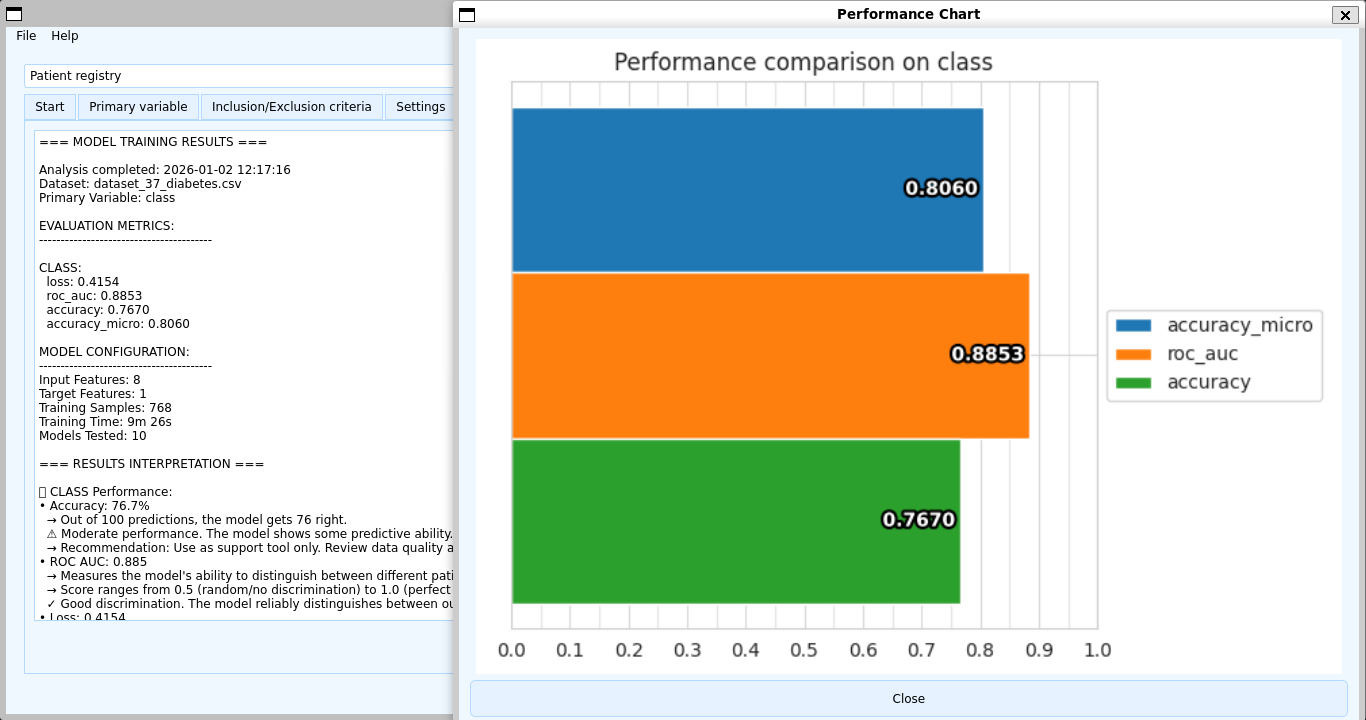
\includegraphics[width=0.92\textwidth]{img/Interface/interface-performance.png}
        \end{figure}
        {\scriptsize Metrics displayed: Accuracy · AUC-ROC · MAE · RMSE · Loss}
      \end{block}
    \end{column}
    \begin{column}{0.5\textwidth}
      \begin{block}{Confusion Matrix}
        \begin{figure}[H]
          \centering
          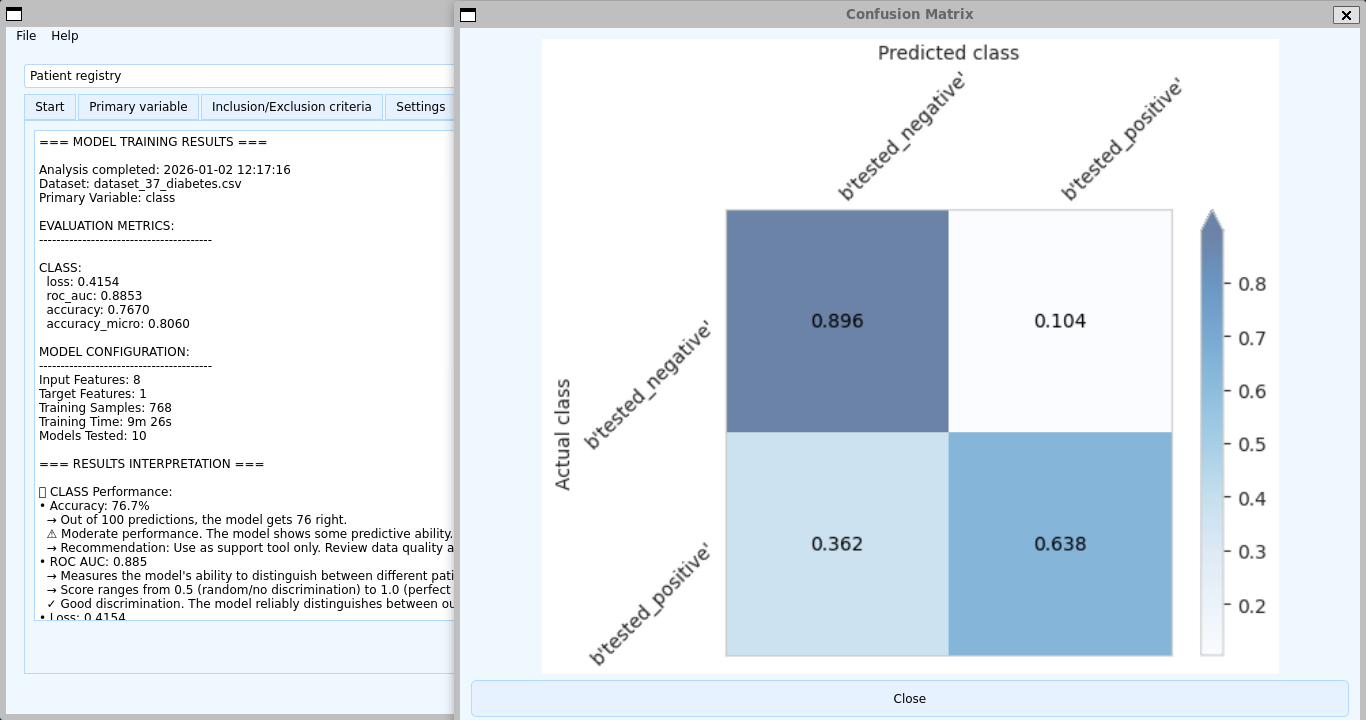
\includegraphics[width=0.85\textwidth]{img/Interface/interface-confusionmatrix.png}
        \end{figure}
        {\scriptsize Visual breakdown enabling clinical interpretation\\
        of false negatives and false positives}
      \end{block}
    \end{column}
  \end{columns}
\end{frame}

% ══════════════════════════════════════════════════════════════════════════════
\section{HGML Alignment}
% ══════════════════════════════════════════════════════════════════════════════

\begin{frame}{HGML Alignment --- Coverage} \small
  \begin{columns}[T]
    \begin{column}{0.54\textwidth}
      \begin{table}
        \centering\tiny
        \renewcommand{\arraystretch}{1.2}
        \begin{tabular}{c p{2.6cm} l}
          \toprule
          \multicolumn{3}{c}{\textbf{Data Use}} \\
          \midrule
          VS4 & Impute missing values        & \cellcolor{UCgreen!25}\textbf{Full} \\
          VR1 & Require incl./excl.\ vars    & \cellcolor{UCgreen!25}\textbf{Full} \\
          IS2 & Select subpopulation         & \cellcolor{UCgreen!25}\textbf{Full} \\
          IS3 & Remove specific instances    & \cellcolor{UCgreen!25}\textbf{Full} \\
          VS1 & Variable selection           & \cellcolor{UCorange!25}\textbf{Partial} \\
          VS3 & Temporal/spatial framing     & \cellcolor{UCorange!25}\textbf{Partial} \\
          VS2 & Create new variables         & \cellcolor{UCred!20}\textbf{Not impl.} \\
          VS5 & Augment data (new sources)   & \cellcolor{UCred!20}\textbf{Not impl.} \\
          IS1 & Select instances to label    & \cellcolor{UCred!20}\textbf{Not impl.} \\
          IS4 & Train/test split control     & \cellcolor{UCred!20}\textbf{Not impl.} \\
          \midrule
          \multicolumn{3}{c}{\textbf{Model Development}} \\
          \midrule
          SD1 & Request data-prep step       & \cellcolor{UCgreen!25}\textbf{Full} \\
          SD2 & Replace data-prep step       & \cellcolor{UCgreen!25}\textbf{Full} \\
          MS1 & Request specific model type  & \cellcolor{UCorange!25}\textbf{Partial} \\
          PT1 & Request specific parameters  & \cellcolor{UCorange!25}\textbf{Partial} \\
          MS2 & Replace model in prior sol.  & \cellcolor{UCred!20}\textbf{Not impl.} \\
          \bottomrule
        \end{tabular}
      \end{table}
    \end{column}
    \begin{column}{0.44\textwidth}
      \begin{table}
        \centering\tiny
        \renewcommand{\arraystretch}{1.2}
        \begin{tabular}{c p{3.2cm} l}
          \toprule
          \multicolumn{3}{c}{\textbf{Model Interpretation}} \\
          \midrule
          QC1 & Request metrics (AUC, MAE\ldots) & \cellcolor{UCgreen!25}\textbf{Full} \\
          QC2 & Intermediate results (hyperopt)  & \cellcolor{UCred!20}\textbf{Not impl.} \\
          MC1 & Compare different models         & \cellcolor{UCred!20}\textbf{Not impl.} \\
          MC2 & Compare on different subsets     & \cellcolor{UCred!20}\textbf{Not impl.} \\
          MC3 & Same model, diff.\ data prep     & \cellcolor{UCred!20}\textbf{Not impl.} \\
          MC4 & Same model, diff.\ parameters    & \cellcolor{UCred!20}\textbf{Not impl.} \\
          MC5 & Two models, all else equal       & \cellcolor{UCred!20}\textbf{Not impl.} \\
          PC1 & Varying parameter ranges         & \cellcolor{UCred!20}\textbf{Not impl.} \\
          \bottomrule
        \end{tabular}
      \end{table}
      \vspace{3mm}
      \begin{block}{\scriptsize Summary}
        \tiny
        \textbf{Data Use}: 4 full · 2 partial · 4 not impl.\\
        \textbf{Model Dev.}: 2 full · 2 partial · 1 not impl.\\
        \textbf{Interpretation}: 1 full · 7 not impl.
      \end{block}
    \end{column}
  \end{columns}
  \vspace{1mm}
  \begin{alertblock}{Main Gap}
    \scriptsize
    The \textbf{comparison category} (MC1--MC5) requires a solution history mechanism
    not yet implemented --- primary HGML limitation of the current system.
  \end{alertblock}
\end{frame}

% ══════════════════════════════════════════════════════════════════════════════
\section{Conclusions}
% ══════════════════════════════════════════════════════════════════════════════

\begin{frame}{Conclusions} \scriptsize
  \begin{block}{Main Contributions}
    \begin{itemize}
      \item \textbf{Novel HGML-grounded system} designed for clinical research
      \item \textbf{Protocol-aware interface}: temporal phases, endpoint hierarchy, inclusion/exclusion logic
      \item \textbf{Strong data-use HGML alignment}: 6/10 tasks fully or partially supported
      \item \textbf{Iterative refinement loop} enabling domain-guided exploration of the modeling space
      \item \textbf{Participatory methodology} grounded in four real protocols and a real clinical dataset
    \end{itemize}
  \end{block}
  \vspace{3mm}
  \begin{block}{Future Work}
  \begin{itemize}
    \item Implement \textbf{solution history mechanism} to enable model comparison (MC1--MC5)
    \item Extend HGML coverage: train/test split control, new variable creation
    \item Broader \textbf{participatory evaluation} with additional CRP profiles
    \item Validation on external clinical datasets beyond the four protocols
  \end{itemize}
    \end{block}
    \vspace{3mm}
  \begin{block}{Take-Home Message}
    Generic AutoML tools fail clinical research not because of lack of ML power, but because
    they ignore the \textbf{semantic structure of clinical data}.
    \\
    HAMELIN's contribution is not a new algorithm. It is a \textbf{new interface paradigm}
    aligned with how clinical research actually works.
  \end{block}
\end{frame}

% ── Thank you ─────────────────────────────────────────────────────────────────
\begin{frame}
  \titlepage
  \vspace{-4mm}
  \begin{center}
    \scriptsize
    \textit{Supported by grant PID2023-146243OB-I00 funded by MICIU/AEI and ERDF/EU}
  \end{center}
\end{frame}

\end{document}